\section{How well it does: images}\label{sec:results-img}

On images v3 runs its image members and the classical ones (\cref{tab:members}); DFG does not run. So on images v3 is v2 with one more member, \code{cgbt}, and a stacker refitted over all members (\cref{sec:image,sec:history}). This section gives v3's test error on the two QuickDraw sets held out for it (\cref{sec:res-img-heldout}) and on the image sets it was developed on (\cref{sec:res-img-dev}). It then asks where the gain over v2 comes from (\cref{sec:res-img-gain}) and what a fit costs (\cref{sec:res-img-compute}).

\paragraph{Sources and rules.} Errors and verdicts come from \repo{study/part10/LEARNER_RESULTS.json}, which \repo{study/part10/compare_learner.py} computes from the result files \texttt{<learner>\_\_<set>.json} in \repo{study/standard_tasks/results/}. Stacking weights, FLOPs and CPU seconds come from the same files and their \texttt{.info.json} records. The tables are generated by \texttt{make\_tables.py} and \cref{fig:images} by \texttt{make\_figures.py}.
\begin{itemize}
\item \emph{Which file is v3.} On \code{qd_c} and \code{qd_d} it is v3's own runs (\code{hyb_portfolio3}). On the development sets it is the frozen image candidate \code{p10_codes}, whose predictions on images are identical to v3's (checked at assembly, \repo{study/part10/hyb_portfolio3/ASSEMBLY.md}).
\item \emph{Cells and verdicts.} A cell is a (set, $n$) pair. The error is measured on the set's fixed 10000-point test set. v3 is \emph{better} or \emph{worse} than a reference at a cell when the errors differ by more than 10\% of the reference's error \emph{and} by more than 2 standard errors; otherwise the cell is a \emph{tie} (\cref{sec:metrics}).
\item \emph{Noise.} At $n=60000$ every learner ran seed 0 only. The standard error is then the test set's binomial noise alone, about 0.34 points at an error of 13\%, so 2 s.e.\ of a difference is about 1.0 point. The 10\% criterion asks for 1.3 points there, so it is the binding one.
\end{itemize}

% ------------------------------------------------------------------------------------------------------------------
\subsection{The held-out sets \code{qd_c} and \code{qd_d}}\label{sec:res-img-heldout}

\code{qd_c} and \code{qd_d} are ten fresh QuickDraw classes each (\cref{sec:tasks}). They were fixed in a commit before any Part 10 design work. No result of a Part 10 learner on them was read before v3 was frozen (\cref{sec:discipline}).
\begin{itemize}
\item \emph{Runs.} v3, v2, v1, \code{hgb}, \code{mlp_strong} and \code{mlp_wide} ran 3 seeds at $n=1000$ and $n=10000$ and seed 0 at $n=60000$. \code{mlp_xl} ran at $n=60000$ only. The control \code{mlp_pool} ran on \code{qd_c} at $n\in\{10000,60000\}$, seed 0. These are the pre-registered cells.
\item \emph{Where to look.} Panel (a) of \cref{tab:img-cells} gives every held-out cell, panel (a) of \cref{tab:img-summary} the verdicts, and \cref{fig:images} the learning curves.
\end{itemize}

\begin{table}[t]
\centering{\scriptsize\setlength{\tabcolsep}{3.4pt}\renewcommand{\arraystretch}{1.12}
\begin{tabular}{lrcccccccccc}
\toprule
set & $n$ & v3 & v2 & v1 & \code{hgb} & \hd{\code{mlp_}\\\code{strong}} & \hd{\code{mlp_}\\\code{wide}} & \hd{\code{mlp_}\\\code{xl}} & \hd{\code{mlp_}\\\code{best+}} & \hd{\code{mlp_}\\\code{pool}} & \code{cnn}\\
\midrule
\multicolumn{12}{l}{\emph{held out for v3 (Part 10): 3 seeds at $n\le10000$, seed 0 at $n=60000$}}\\
\code{qd_c} & 1000 & \textbf{26.58} & 27.48\rlap{$^{\circ}$} & 31.68 & 37.52 & 33.01 & 33.02 & -- & 33.01 & -- & 24.36\rlap{$^{\circ}$}\\
\code{qd_c} & 10000 & \textbf{16.17} & 17.79\rlap{$^{\circ}$} & 20.05 & 22.76 & 20.94 & 20.41 & -- & 20.41 & 19.37 & 14.84\rlap{$^{\circ}$}\\
\code{qd_c} & 60000 & \textbf{12.76} & 13.63\rlap{$^{\circ}$} & 15.77 & 18.22 & 16.08 & 14.12\rlap{$^{\circ}$} & 14.12\rlap{$^{\circ}$} & 14.12\rlap{$^{\circ}$} & 14.48 & --\\
\addlinespace[2pt]
\code{qd_d} & 1000 & \textbf{26.12} & 26.71\rlap{$^{\circ}$} & 30.21 & 35.33 & 31.62 & 31.40 & -- & 31.40 & -- & --\\
\code{qd_d} & 10000 & \textbf{16.38} & 17.82\rlap{$^{\circ}$} & 19.70 & 21.85 & 20.30 & 19.89 & -- & 19.89 & -- & --\\
\code{qd_d} & 60000 & \textbf{12.64} & 13.99\rlap{$^{\circ}$} & 15.97 & 17.48 & 15.34 & 14.31 & 13.83\rlap{$^{\circ}$} & 13.83\rlap{$^{\circ}$} & -- & --\\
\bottomrule
\end{tabular}
}
\caption{Test error (\%) on every image cell with a v3 result \status{Numerical}. Seed mean of 3 at $n\le10000$ and seed 0 at $n=60000$, except where a panel says otherwise. \code{mlp_xl}, \code{mlp_pool} and \code{cnn} are seed 0 everywhere. Bold: the lowest error among v3, v2, v1, \code{hgb}, \code{mlp_strong}, \code{mlp_wide} and \code{mlp_xl}. A reference's entry carries $^{\circ}$ where the cell is a tie with v3 and $^{\ast}$ where the reference is clearly better than v3. An unmarked entry is clearly worse than v3. ``--'': not run (yet). \code{mlp_best+} is the per-cell minimum over all MLP references, and it is defined only at the $n$ where the Part 7 \code{mlp} has run. \code{mlp_pool} is \code{mlp_strong} given v2's pooled sums (a control). \code{cnn} sees the unpermuted pixels (context, not a reference). Panel (b): v3 is seed 0 and the references are seed means. Panel (c): v3 and v2 are seed 0, and \code{mlp_strong}, \code{hgb} and v1 are seed means. ``Fashion'' is Fashion-MNIST. Source: \repo{study/part10/LEARNER_RESULTS.json}; markers by \code{compare_hybrid.cells}.}
\label{tab:img-cells}
\end{table}

\begin{table}[t]
\centering{\footnotesize\setlength{\tabcolsep}{5pt}
\begin{tabular}{llccc}
\toprule
sets & reference & $n$ & cells (better / tie / worse) & mean $\log_2$ ratio\\
\midrule
\code{qd_c}, \code{qd_d} & \code{mlp_strong} & all & 6 (6/0/0) & $-0.314$\\
 &  & $\le3000$ & 2 (2/0/0) & $-0.294$\\
 &  & $\ge10000$ & 4 (4/0/0) & $-0.324$\\
 & \code{mlp_wide} & all & 6 (5/1/0) & $-0.253$\\
 &  & $\le3000$ & 2 (2/0/0) & $-0.289$\\
 &  & $\ge10000$ & 4 (3/1/0) & $-0.235$\\
 & \code{mlp_xl} & all & 2 (0/2/0) & $-0.138$\\
 &  & $\ge10000$ & 2 (0/2/0) & $-0.138$\\
 & \code{mlp_best} & all & 2 (2/0/0) & $-0.343$\\
 &  & $\le3000$ & 1 (1/0/0) & $-0.313$\\
 &  & $\ge10000$ & 1 (1/0/0) & $-0.373$\\
 & \code{mlp_best+} & all & 2 (2/0/0) & $-0.325$\\
 &  & $\le3000$ & 1 (1/0/0) & $-0.313$\\
 &  & $\ge10000$ & 1 (1/0/0) & $-0.336$\\
 & v2 & all & 6 (0/6/0) & $-0.097$\\
 &  & $\le3000$ & 2 (0/2/0) & $-0.040$\\
 &  & $\ge10000$ & 4 (0/4/0) & $-0.125$\\
 & v1 & all & 3 (3/0/0) & $-0.271$\\
 &  & $\le3000$ & 1 (1/0/0) & $-0.210$\\
 &  & $\ge10000$ & 2 (2/0/0) & $-0.302$\\
 & \code{mlp_pool} (control) & all & 2 (2/0/0) & $-0.222$\\
 &  & $\ge10000$ & 2 (2/0/0) & $-0.222$\\
\midrule
\code{qd_a}, \code{qd_b}$^c$ & \code{mlp_strong} & all & 5 (5/0/0) & $-0.337$\\
 &  & $\le3000$ & 2 (2/0/0) & $-0.338$\\
 &  & $\ge10000$ & 3 (3/0/0) & $-0.337$\\
 & \code{mlp_wide} & all & 5 (5/0/0) & $-0.302$\\
 &  & $\le3000$ & 2 (2/0/0) & $-0.320$\\
 &  & $\ge10000$ & 3 (3/0/0) & $-0.291$\\
 & \code{mlp_xl} & all & 1 (1/0/0) & $-0.204$\\
 &  & $\ge10000$ & 1 (1/0/0) & $-0.204$\\
 & \code{mlp_best} & all & 5 (5/0/0) & $-0.337$\\
 &  & $\le3000$ & 2 (2/0/0) & $-0.338$\\
 &  & $\ge10000$ & 3 (3/0/0) & $-0.337$\\
 & \code{mlp_best+} & all & 5 (5/0/0) & $-0.294$\\
 &  & $\le3000$ & 2 (2/0/0) & $-0.320$\\
 &  & $\ge10000$ & 3 (3/0/0) & $-0.276$\\
 & \code{hgb} & all & 5 (5/0/0) & $-0.443$\\
 &  & $\le3000$ & 2 (2/0/0) & $-0.419$\\
 &  & $\ge10000$ & 3 (3/0/0) & $-0.460$\\
 & v2 & all & 5 (0/5/0) & $-0.089$\\
 &  & $\le3000$ & 2 (0/2/0) & $-0.064$\\
 &  & $\ge10000$ & 3 (0/3/0) & $-0.107$\\
 & v1 & all & 5 (5/0/0) & $-0.286$\\
 &  & $\le3000$ & 2 (2/0/0) & $-0.246$\\
 &  & $\ge10000$ & 3 (3/0/0) & $-0.314$\\
 & \code{mlp_pool} (control) & all & 3 (3/0/0) & $-0.204$\\
 &  & $\ge10000$ & 3 (3/0/0) & $-0.204$\\
 & \code{cnn} (context) & all & 1 (0/0/1) & $+0.245$\\
 &  & $\ge10000$ & 1 (0/0/1) & $+0.245$\\
\bottomrule
\end{tabular}
}
\caption{v3 against each image reference \status{Numerical}. ``Cells'' counts the (set, $n$) pairs compared, with v3 better / tied / worse by the cell rule (\cref{sec:metrics}). ``Mean $\log_2$ ratio'' is the mean over those cells of $\log_2$(v3's error / the reference's error); negative means v3 is lower. \code{mlp_best} is the per-cell minimum over the Part 7--8 MLP variants (\code{mlp}, its regularized versions, \code{mlp_strong} and its single network \code{mlp_strong1}). \code{mlp_best+} adds \code{mlp_wide}, its single network \code{mlp_wide1}, and \code{mlp_xl}. Both are defined only where the Part 7 \code{mlp} has run. Panels (b) and (c) compare single v3 fits (seed 0) with the references' seed means. Source: \repo{study/part10/LEARNER_RESULTS.json}.}
\label{tab:img-summary}
\end{table}

\begin{figure}[tbp]
\centering
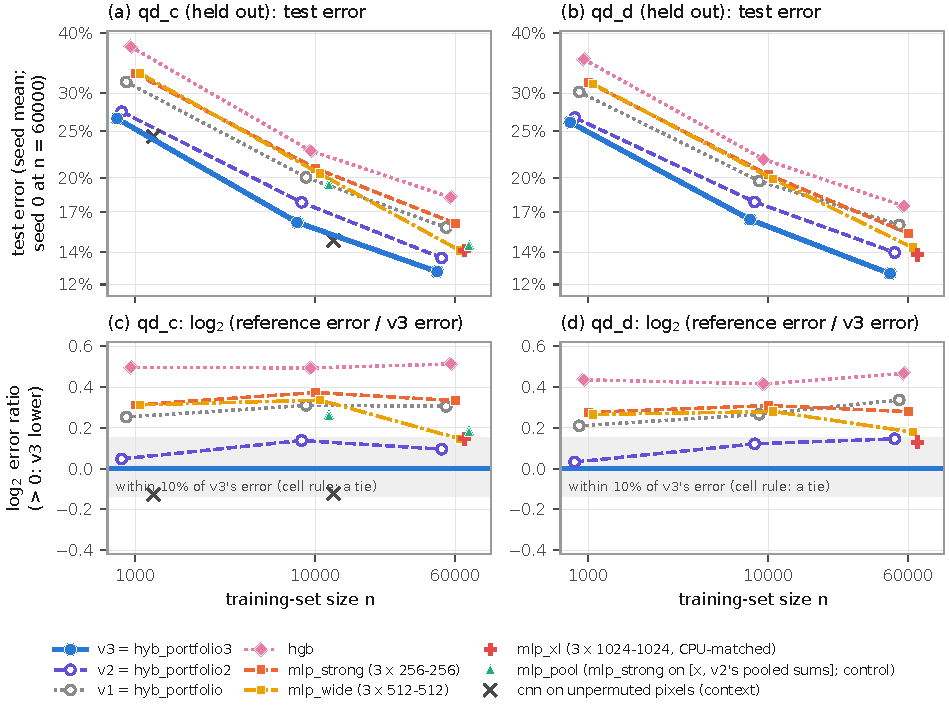
\includegraphics[width=\textwidth]{figures/fig_images.pdf}
\caption{The held-out QuickDraw sets \status{Numerical}. Top: test error against $n$ (log--log; seed mean of 3 at $n\le10000$, seed 0 at $n=60000$; \code{mlp_xl}, \code{mlp_pool} and \code{cnn} seed 0). Bottom: each reference's error relative to v3's at the same $n$, as $\log_2$(reference error / v3 error), so points above 0 are cells where v3 is lower. In the grey band the two errors are within 10\% of each other, and the cell rule calls the cell a tie whatever the noise. Markers are shifted slightly sideways so that they do not hide each other. Generated by \texttt{make\_figures.py} (\texttt{fig\_images}) from the result files; the plotted values are in \texttt{figures/fig\_images.json}.}
\label{fig:images}
\end{figure}

\paragraph{Against the MLP references} \status{Numerical}. At all six held-out cells v3's error is lower than every reference's and the control's.
\begin{itemize}
\item \code{mlp_strong} (ensemble of three 256-256 networks): v3 is clearly better at all 6 cells. Its error is 17--23\% lower, and the mean $\log_2$ ratio is $-0.31$ ($-0.32$ at $n\ge10000$).
\item \code{mlp_wide} (three 512-512 networks): clearly better at 5 cells. The sixth, \code{qd_c} at $n=60000$, is a tie: 12.76\% against 14.12\%, 9.6\% lower, just inside the 10\% threshold. Mean $-0.25$.
\item \code{mlp_xl} (three 1024-1024 networks, the CPU-matched reference; $n=60000$ only): two ties. v3 is 9.6\% lower on \code{qd_c} (12.76\% against 14.12\%) and 8.6\% lower on \code{qd_d} (12.64\% against 13.83\%). Mean $-0.14$.
\item \code{mlp_best} and \code{mlp_best+} are defined so far only on \code{qd_c} at $n=1000$ and $n=10000$, because the Part 7 \code{mlp} has run only up to $n=10000$ there. v3 is clearly better at both cells.
\end{itemize}
\todo{The Part 7 mlp on qd\_c ($n\ge30000$) and on qd\_d is still running. When it lands, mlp\_best and mlp\_best+ cover more cells: update this item and panel (a) of the summary table.}

So at $n\le10000$ v3 is clearly better than every MLP reference. At $n=60000$ the two widest ensembles come within 10\% of it on \code{qd_c}, and \code{mlp_xl} also on \code{qd_d}.

\paragraph{Against the other references} \status{Numerical}.
\begin{itemize}
\item \code{hgb} (on \code{qd_c} so far): v3 is clearly better at all 3 cells, with errors 29--30\% lower (mean $\log_2$ ratio $-0.50$).
\item v1, the Part 8 portfolio (on \code{qd_d} so far): clearly better at all 3 cells, by 13.5\%, 16.9\% and 20.9\% at $n=1000$, 10000 and 60000.
\item v2: all 6 cells are ties. v3's error is lower at every cell, by 2.2--3.3\% at $n=1000$ and by 6.4--9.6\% at $n\ge10000$, but never by more than 10\%. The mean $\log_2$ ratio is $-0.10$, and $-0.125$ at $n\ge10000$.
\end{itemize}
\todo{hgb on qd\_d and v1 on qd\_c are still running. When they land, update these two items (counts and ranges) and the summary table.}

\paragraph{The control and the context} \status{Numerical}.
\begin{itemize}
\item \code{mlp_pool} is \code{mlp_strong} given v2's pooled subset sums as extra inputs (seed 0, \code{qd_c} only). v3 is clearly better at both cells: 16.17\% against 19.37\% at $n=10000$, and 12.76\% against 14.48\% at $n=60000$. v2 ties it at both cells (17.79\% and 13.63\%, which are 8.2\% and 5.9\% lower), as it did on \code{qd_a} and \code{qd_b} in Part 9. This control matches v2's representation, not v3's: no MLP was given the bar sums (\cref{sec:res-img-gain}).
\item \code{cnn}, a small convolutional network on the unpermuted pixels, is context, not a reference. Its \code{qd_c} runs ($n=1000$ and 10000) are still in progress.
\end{itemize}
\todo{cnn on qd\_c is running: add its two cells here and in the tables (context only; on qd\_a at $n=10000$ it was better than v3, \cref{sec:res-img-dev}).}

\paragraph{The best-learner rule}\label{sec:res-img-rule} \status{Numerical}. The pre-registered rule does not use cell verdicts (\cref{sec:discipline}). It makes v3 the learner of this paper if two conditions hold:
\begin{itemize}
\item the mean $\log_2$ error ratio of v3 to v2 over the four held-out image cells with $n\ge10000$ is below 0. It is $-0.125$: the cells give $-0.138$ and $-0.095$ on \code{qd_c} ($n=10000$, 60000) and $-0.122$ and $-0.146$ on \code{qd_d};
\item the mean $\log_2\nstar$ ratio of v3 to v2 on \code{dlheld7} is at most $+0.1$. It is $-0.004$ (\cref{sec:res-dlheld7}).
\end{itemize}
Both hold, so v3 replaced v2. The rule was applied by \repo{study/part10/compare_part10.py} (\repo{study/part10/RESULTS.md}) after every held-out cell of v3 and v2 was in, and the decision is recorded in \repo{study/part10/PROTOCOL.md} (28 October, 04:25 UTC).

\paragraph{How firm the gain over v2 is.} By the cell rule it is not established at any single cell. Its direction is consistent: in all 14 seed-paired fits (same training sample, same test set), v3's error is below v2's, by 0.47 to 1.86 points \status{Numerical}. This is a description made after the results were in, not a pre-registered test. The 14 fits share two test sets, so they are not independent.

% ------------------------------------------------------------------------------------------------------------------
\subsection{The other image sets: development data for v3}\label{sec:res-img-dev}

Panels (b) and (c) of \cref{tab:img-cells,tab:img-summary} give v3 at the cells of its fixed development evaluation. These sets are not held out for v3, and the cells are in-sample for a choice:
\begin{itemize}
\item \emph{Tuning.} The image builders tuned on validation rows of the training pools of \code{qd_dev}, \code{qd_a} and Fashion-MNIST, never on a test set. \code{qd_b} was not used in \code{p10_codes}'s development (\repo{study/part10/p10_codes/DESIGN.md}).
\item \emph{Selection.} After each freeze, the candidate's test error was computed once at 8 cells: \code{qd_dev} and Fashion-MNIST at $n\in\{1000,10000\}$, and \code{qd_a} and \code{qd_b} at $n\in\{3000,10000\}$. A ninth cell, \code{qd_a} at $n=60000$, was added as a check. The integration rule then used these test errors to qualify the two candidates and choose between them (\repo{study/part10/RESULTS.md}).
\item \emph{The choice.} \code{p10_codes} had a mean $\log_2$ ratio against v2 of $-0.078$ over the 8 cells, and at \code{qd_a}, $n=60000$, 10.82\% error, 1453 CPU s and 0.58 of the FLOP budget. \code{p10_hier} had $-0.071$, 11.08\%, 924 s and 0.44. The rule took the lower mean.
\end{itemize}
The v3 numbers here are therefore the errors of the candidate that these very numbers selected. With two candidates this close the selection effect is small, but these cells are not a test of v3. Each v3 entry is one fit (seed 0).

\paragraph{\code{qd_a} and \code{qd_b}} (held out in Part 9) \status{Numerical}.
\begin{itemize}
\item \emph{References.} v3 is clearly better than \code{mlp_strong}, \code{mlp_wide}, \code{hgb} and v1 at all 5 cells. It is also clearly better than \code{mlp_xl} at \code{qd_a}, $n=60000$ (10.82\% against 12.46\%, 13.2\% lower), and than \code{mlp_pool} at the 3 cells where both were run (at \code{qd_a}, $n=60000$: 10.82\% against 12.25\%).
\item \emph{v2.} All 5 cells are ties, with v3 2.6--9.6\% lower (mean $\log_2$ ratio $-0.089$). Here v2's entries are seed means. Against v2's seed-0 fits, as the integration rule compared them, the margins are similar: for example 17.48\% against 18.75\% at \code{qd_a}, $n=3000$.
\item \emph{The context.} The \code{cnn} on unpermuted pixels is the only learner better than v3: 12.00\% against 14.22\% at \code{qd_a}, $n=10000$, an error 18.5\% lower. Among v3's cells, only the one at $n=60000$ (10.82\%) is below it.
\item \emph{Comparison with Part 9.} At $n=60000$, v2 tied \code{mlp_xl} on both sets (11.97\% against 12.46\% on \code{qd_a}; 14.88\% against 14.79\% on \code{qd_b}). The control \code{mlp_pool} matched v2 (12.25\% and 14.74\%). v3's \code{qd_a} cell (10.82\%) is clearly better than both. v3 was not run at \code{qd_b}, $n=60000$.
\end{itemize}

\paragraph{\code{qd_dev} and Fashion-MNIST} (development throughout) \status{Numerical}.
\begin{itemize}
\item \emph{\code{qd_dev}.} v3 is clearly better than \code{mlp_strong}, \code{hgb} and v1 at both cells, for example 13.30\% against \code{mlp_strong}'s 17.49\% at $n=10000$. It ties v2 at both cells (21.18\% against 22.22\%, 13.30\% against 14.63\%).
\item \emph{Fashion-MNIST.} Every comparison is a tie. v3 has 17.97\% and 12.38\% against \code{mlp_strong}'s 18.60\% and 12.64\% (3.4\% and 2.0\% lower). It also ties v2, v1 and \code{hgb}. This is the set where the bars do not help. On the builder's validation rows, a booster on \code{cgbt}'s bank was worse there than one on v2's bank (18.30\% against 17.74\% at $n=1000$; \repo{study/part10/p10_codes/DESIGN.md}, \S4.2). \code{cgbt}'s stacking weight is 0.05 and 0.07 there, against 0.23--0.50 on the QuickDraw development cells.
\item \emph{Larger $n$.} v3 was not run on Fashion-MNIST beyond $n=10000$. v2's image path (\code{p9_gates}, Part 9, seed 0) reached 9.64\% at $n=60000$, against \code{mlp_strong}'s 9.66\%.
\item \emph{A threading caveat.} v2's own cells on these two sets were run with multi-threaded BLAS, while every v3 and held-out run is single-threaded. A single-threaded refit of v2 at \code{qd_dev}, $n=10000$, gives 14.67\% instead of 14.63\% (\repo{study/part10/PROTOCOL.md}, note).
\end{itemize}

% ------------------------------------------------------------------------------------------------------------------
\subsection{Where the gain over v2 comes from}\label{sec:res-img-gain}

\begin{table}[t]
\centering{\scriptsize\setlength{\tabcolsep}{3.3pt}
\begin{tabular}{lrccccccccccccc}
\toprule
 & & \multicolumn{5}{c}{v3: stacking weight} & \multicolumn{4}{c}{v2: stacking weight} & \multicolumn{4}{c}{out-of-fold error (\%)}\\
\cmidrule(lr){3-7}\cmidrule(lr){8-11}\cmidrule(lr){12-15}
set & $n$ & \code{cgbt} & \code{ggbt} & \code{gknn} & \code{knn} & rest & \code{ggbt} & \code{gknn} & \code{knn} & rest & \code{cgbt} & \code{ggbt} & v3 & v2\\
\midrule
\code{qd_c} & 1000 & 0.27 & 0.02 & 0.38 & 0.15 & 0.03 & 0.24 & 0.46 & 0.17 & 0.04 & 30.8 & 32.5 & 27.6 & 29.0\\
\code{qd_c} & 10000 & 0.36 & 0.04 & 0.15 & 0.15 & 0.01 & 0.35 & 0.24 & 0.18 & 0.03 & 16.8 & 18.9 & 16.2 & 17.2\\
\code{qd_c} & 60000 & 0.49 & 0.12 & 0.11 & 0.17 & 0.00 & 0.50 & 0.20 & 0.24 & 0.00 & 13.3 & 14.6 & 12.8 & 13.5\\
\code{qd_d} & 1000 & 0.23 & 0.08 & 0.30 & 0.18 & 0.03 & 0.27 & 0.35 & 0.21 & 0.04 & 28.1 & 29.8 & 26.3 & 26.1\\
\code{qd_d} & 10000 & 0.39 & 0.01 & 0.13 & 0.19 & 0.01 & 0.29 & 0.20 & 0.26 & 0.10 & 17.1 & 19.2 & 16.2 & 17.3\\
\code{qd_d} & 60000 & 0.45 & 0.12 & 0.04 & 0.12 & 0.00 & 0.50 & 0.11 & 0.23 & 0.00 & 12.6 & 14.3 & 12.5 & 13.5\\
\bottomrule
\end{tabular}
}
\caption{What carries v3 and v2 on the held-out image sets \status{Numerical}. Left: stacking weight per member family (seed mean of 3 fits at $n\le10000$; one fit at $n=60000$). \code{gknn}: $k$-NN votes on the pooled sums. \code{knn}: $k$-NN votes on the pixels. ``rest'': Part 8's \code{gbt}, \code{et} and \code{lin}; \code{lin} has weight 0 in every fit here. Right: out-of-fold error on the training rows of the two boosters and of the whole stack (5-fold at $n\le3000$; one holdout of 2000 rows at $n=10000$ and 6000 rows at $n=60000$). \code{ggbt}'s out-of-fold error is the same in v3 and v2 in every fit. The weights multiply log-probabilities of different calibration, so they are not shares of the decision. Source: \texttt{hyb\_portfolio\{3,2\}\_\_qd\_\{c,d\}.info.json} in \repo{study/standard_tasks/results/}.}
\label{tab:img-stack}
\end{table}

\paragraph{The same members, plus one} \status{Numerical}. In each of the 14 held-out fits, v3's and v2's records give every shared member the same out-of-fold error, and \code{ggbt} the same number of boosting rounds. \code{cgbt} draws from its own random stream, so v3's other members are v2's fits. v3 and v2 therefore differ only by \code{cgbt} and by the stacking weights. The final refits also differ where a weight moves between zero and a positive value, because a member with weight 0 is not refitted. \Cref{tab:img-stack} gives the weights and the out-of-fold errors.
\begin{itemize}
\item \emph{\code{cgbt} is the better booster.} Its out-of-fold error is below \code{ggbt}'s in all 14 fits: by 0.2--4.0 points at $n=1000$, and by 0.13--0.20 in $\log_2$ at $n\ge10000$. It is the lowest of all members in 13 of the 14 fits. The exception is \code{qd_c}, $n=1000$, seed 1, where $k$-NN on pooled sums is lower (30.1\% against 31.8\%).
\item \emph{It takes \code{ggbt}'s place in the stack.} At $n\ge10000$, \code{cgbt} has the largest family weight in all 8 fits (0.32--0.49). \code{ggbt}'s weight falls from 0.25--0.50 in v2 to 0--0.12 in v3. At $n=1000$, the $k$-NN votes on pooled sums keep the largest family weight in 5 of 6 fits, in v3 as in v2.
\item \emph{The stack improves.} v3's stacked out-of-fold error is below v2's in 12 of the 14 fits. At \code{qd_d}, $n=1000$, it is equal in one fit and higher in one (27.2\% against 26.3\%).
\end{itemize}
Two cautions about the weights apply (\cref{sec:interp-img}). They multiply log-probabilities of different calibration: boosters stopped early on error are over-confident, while $k$-NN votes are smooth. And the convex stacker splits weight between two nearly collinear boosters on one holdout. So ``\code{ggbt} gets weight 0'' describes one fit, not a property of the learner.

\paragraph{What \code{cgbt} changes: the bank, not the schedule} \status{Numerical}. \code{cgbt} has \code{ggbt}'s tree settings and early-stopping rule. It differs from \code{ggbt} in three ways: its bank adds bar sums at two lengths, it drops the 300 prototype-pair projections, and its per-tree column fraction is 0.05 instead of 0.12 (\cref{sec:image}). The builder's development runs separate these effects (one booster alone, $n=5000$, validation rows, seed 0; \repo{study/part10/p10_codes/DESIGN.md}, \S4.2). On \code{qd_dev}:
\begin{itemize}
\item v2's bank gave 17.66\% error, and dropping the pairs gave 17.20\%;
\item adding the bars at both lengths gave 15.92\%, and the lower column fraction then gave 15.82\%.
\end{itemize}
On \code{qd_a} the full change gave 17.68\% $\to$ 16.78\%. So on QuickDraw most of the gain is the bars. On Fashion-MNIST the bars did not help. In \code{cgbt}'s fitted trees the bars, two thirds of its columns, carry 0.72--0.80 of the split gain on QuickDraw and MNIST (development fits; \cref{sec:interp-img}). Split gain describes how the trees split, not what the predictions depend on.

\paragraph{Compared with Part 9} \status{Numerical}. In Part 9, at $n=60000$ on \code{qd_a} and \code{qd_b}, v2 tied the CPU-matched \code{mlp_xl}, and the control \code{mlp_pool} matched v2. Most of v2's large-$n$ advantage over the MLPs was therefore the pooled-sum representation, which an MLP uses as well as the trees do. The Part 10 held-out sets repeat this for v2:
\begin{itemize}
\item v2 ties \code{mlp_xl} at $n=60000$ on both sets (13.63\% against 14.12\%; 13.99\% against 13.83\%);
\item v2 ties \code{mlp_pool} at both \code{qd_c} cells.
\end{itemize}
v3 moves past the control: it is clearly better than \code{mlp_pool} at both cells, by 16.5\% and 11.9\%. Against \code{mlp_xl} it is 9.6\% and 8.6\% lower, just inside the 10\% threshold.

\paragraph{Reading} \status{Heuristic}. On images v3's gain over v2 is a better fixed representation for gradient-boosted trees: sums over short runs of pixels along lines recovered from pixel correlations, used at fixed positions. Recovering the image topology from such correlations is an old idea \cite{leroux2007topology}, and so is grouping inputs into receptive fields by their correlations \cite{coates2011receptive}. The gain is not evidence that discrete search beats gradient-based learning on images, for three reasons.
\begin{itemize}
\item \emph{The control for v3's own representation was not run.} No MLP was given the bar sums as well as the pooled sums. Part 9's control matched v2 once it had v2's features, so part of v3's margin over the MLPs may again be available to a network given the same features.
\item \emph{Gradient-trained networks that learn local structure were not run.} For example, an MLP trained to learn sparse local connectivity \cite{neyshabur2020convolutions} would be the information-matched comparison.
\item \emph{A network told the layout is better.} At the one cell where both have run, the small \code{cnn} has 12.00\% error against v3's 14.22\% (\code{qd_a}, $n=10000$).
\end{itemize}
What v3 shows is narrower: a learner that never reads the pixel layout, and whose features are fixed subset sums chosen by rank statistics, reaches 12.6--12.8\% error on fresh QuickDraw classes at $n=60000$. That is 8.6--9.6\% below a CPU-matched MLP ensemble, a tie by the cell rule, and clearly below an MLP given v2's representation (\code{qd_c}).

% ------------------------------------------------------------------------------------------------------------------
\subsection{Compute}\label{sec:res-img-compute}

\begin{table}[t]
\centering{\scriptsize\setlength{\tabcolsep}{3.2pt}
\begin{tabular}{lrccccccccc}
\toprule
 & & \multicolumn{2}{c}{FLOPs / budget} & \multicolumn{3}{c}{CPU s per fit} & \multicolumn{4}{c}{MLP references: wall s per fit (FLOPs / budget)}\\
\cmidrule(lr){3-4}\cmidrule(lr){5-7}\cmidrule(lr){8-11}
set & $n$ & v3 & v2 & v3 & \hd{of which\\\code{cgbt}} & v2 & \code{mlp_strong} & \code{mlp_wide} & \code{mlp_xl} & \code{mlp_pool}\\
\midrule
\code{qd_c} & 1000 & 0.49--0.51 & 0.35 & 229--256 & 120--132 & 144--166 & 384 (2.0) & 249 (5.0) & -- & --\\
\code{qd_c} & 10000 & 0.34--0.48 & 0.22--0.26 & 513--785 & 251--430 & 284--440 & 490 (2.0) & 396 (5.0) & -- & 333 (5.9)\\
\code{qd_c} & 60000 & 0.57 & 0.42 & 1361 & 668 & 1296 & 963 (2.0) & 1168 (5.0) & 2196 (9.2) & 716 (5.9)\\
\addlinespace[2pt]
\code{qd_d} & 1000 & 0.50--0.51 & 0.35 & 266--291 & 128--140 & 162--175 & 98 (2.0) & 248 (5.0) & -- & --\\
\code{qd_d} & 10000 & 0.30--0.46 & 0.24--0.29 & 402--768 & 233--377 & 394--602 & 152 (2.0) & 440 (5.0) & -- & --\\
\code{qd_d} & 60000 & 0.58 & 0.42 & 1464 & 760 & 1531 & 422 (2.0) & 989 (5.0) & 1335 (9.2) & --\\
\bottomrule
\end{tabular}
}
\caption{Compute per fit on the held-out image cells \status{Numerical}. Budget: three training runs of the baseline MLP (\code{common.budget_real}), $1.24$, $2.42$ and $6.21\times10^{12}$ FLOPs at $n=1000$, 10000 and 60000. FLOPs / budget: each learner's own count, everything in the fit included and prediction excluded. CPU s: process CPU seconds per fit, and the seconds v3 attributes to \code{cgbt}. A range is over the 3 seeds; $n=60000$ has one fit. The MLP references record wall-clock seconds per fit on the shared 4-core machine, not process CPU time (the \texttt{cpu\_seconds} field of their result files), with their FLOPs per fit in units of the budget in brackets. Sources: the result files and \texttt{.info.json} records in \repo{study/standard_tasks/results/}.}
\label{tab:img-compute}
\end{table}

\paragraph{FLOPs} \status{Numerical}. The budget of a real-data fit is three training runs of the baseline MLP: $1.24\times10^{12}$ FLOPs at $n=1000$, $2.42\times10^{12}$ at $n=10000$ and $6.21\times10^{12}$ at $n=60000$ (\cref{tab:img-compute}).
\begin{itemize}
\item \emph{v3 and v2.} By its own count v3 uses 0.30--0.58 of the budget on the held-out cells, the most at $n=60000$. v2 uses 0.22--0.42. \code{cgbt} adds 0.05--0.22.
\item \emph{Near the guard at $n=3000$.} On the development sets, at $n=3000$ (no held-out cell has this size), v3 used 0.85 of the budget on \code{qd_a} and on \code{qd_b}. That is close to the guard at 0.9, which skips members whose projected cost would exceed it (\cref{sec:portfolio}). Part 9's compute audit found that the FLOP charge of Part 8's \code{gbt} member is too low by a factor of 1.14--1.46 at this size, and it projected v2's $n=3000$ QuickDraw cells at about 0.72 (0.69--0.81) of the budget, against v2's own count of at most 0.62. v3 keeps that charge, and no compute audit was made of v3. Applying the audit's factor to \code{gbt} alone (0.28 of the budget by v3's count) puts these two cells at 0.88--0.98 \status{Heuristic}. So v3 is within the budget at $n=3000$ by its own count, but not with a clear margin.
\item \emph{The MLP references.} Every MLP reference spends more FLOPs than the budget: \code{mlp_strong} 2.0 budgets per fit (six training runs), \code{mlp_wide} 5.0, \code{mlp_pool} 5.9 and \code{mlp_xl} 9.2. So by FLOPs v3 is cheaper than every MLP reference at every cell, by a factor of at least 3.4 (\code{mlp_strong} at \code{qd_d}, $n=60000$).
\end{itemize}

\paragraph{CPU time} \status{Numerical}. Equal FLOPs are far from equal CPU time.
\begin{itemize}
\item \emph{v3 and v2.} A v3 fit takes 229--291 CPU s at $n=1000$, 402--785 s at $n=10000$, and 1361 and 1464 s at $n=60000$. v2 takes 144--175, 284--602, and 1296 and 1531 s.
\item \emph{Why v3 is not slower at $n=60000$.} There v3 takes about as long as v2 (1.05$\times$ on \code{qd_c}, 0.96$\times$ on \code{qd_d}), although it fits a second booster. \code{cgbt} takes 668 and 760 s. But v3's \code{ggbt} takes 482 and 474 s against v2's 1091 and 1305 s. The reason is that v3 sets LightGBM's column-wise layout, which leaves the predictions unchanged (\repo{study/part10/p10_codes/DESIGN.md}, \S1). Part 9 found this fix but did not apply it to v2.
\item \emph{A like-for-like estimate.} The comparison with v2 is not like for like. v3's time minus \code{cgbt}'s, 693 and 704 s, estimates v2 with the same layout. By that estimate the second booster about doubles the CPU time of a fit at $n=60000$.
\item \emph{The MLP references.} At $n=60000$ they take 963 and 422 s of wall time (\code{mlp_strong}), 1168 and 989 s (\code{mlp_wide}) and 2196 and 1335 s (\code{mlp_xl}); \code{mlp_pool} takes 716 s. So \code{mlp_xl} takes about as long as v3, which is the sense in which it is CPU-matched. The other ensembles take 0.3--0.9 of v3's time.
\item \emph{How rough the MLP times are.} They are wall-clock seconds on the shared machine, and they vary with the load from concurrent jobs. The same \code{mlp_strong} recipe took 384 s per fit at \code{qd_c}, $n=1000$, and 98 s at \code{qd_d}, $n=1000$. In Part 9 it took 28 s at \code{qd_a}.
\end{itemize}

\paragraph{Prediction} is not charged for any learner. A v2 query costs about $2.8\times10^8$ FLOPs at $n=60000$, about $500\times$ an MLP's, because the $k$-NN members scan the training set (Part 9). v3 adds \code{cgbt}'s bank projection, about $1.2\times10^7$ FLOPs per query, and up to about 4000 more tree traversals (\repo{study/part10/p10_codes/DESIGN.md}, \S6).

% ------------------------------------------------------------------------------------------------------------------
\paragraph{Summary of the image results.}
\begin{itemize}
\item \emph{Strong points} \status{Numerical}. On the two held-out sets v3 is clearly better than \code{mlp_strong} at every cell, and than every MLP reference at $n\le10000$. It is clearly better than the control \code{mlp_pool} at both cells where that was run. Its error is below every reference's at every held-out cell.
\item \emph{Weak points} \status{Numerical}. At $n=60000$ the CPU-matched \code{mlp_xl} is within 10\% of v3 on both sets (two ties), and \code{mlp_wide} on \code{qd_c}. v3's gain over v2 is below the cell rule's threshold at every cell; the best-learner rule, which uses mean $\log_2$ ratios, still prefers v3. On Fashion-MNIST v3 is level with \code{mlp_strong}. The \code{cnn} that sees the layout is better at the one cell where both have run. A fit takes 23--24 CPU minutes at $n=60000$. The FLOP count reaches 0.85 of the budget at $n=3000$, and with Part 9's audited correction it would be close to 1.
\item \emph{What it means} \status{Heuristic}. The gain over v2 comes from a richer fixed feature bank for gradient-boosted trees, not from a new kind of learning. Whether an MLP would gain as much from the same bank was not tested.
\end{itemize}
